\documentclass[]{article}
\usepackage{lmodern}
\usepackage{amssymb,amsmath}
\usepackage{ifxetex,ifluatex}
\usepackage{fixltx2e} % provides \textsubscript
\ifnum 0\ifxetex 1\fi\ifluatex 1\fi=0 % if pdftex
  \usepackage[T1]{fontenc}
  \usepackage[utf8]{inputenc}
\else % if luatex or xelatex
  \ifxetex
    \usepackage{mathspec}
    \usepackage{xltxtra,xunicode}
  \else
    \usepackage{fontspec}
  \fi
  \defaultfontfeatures{Mapping=tex-text,Scale=MatchLowercase}
  \newcommand{\euro}{€}
\fi
% use upquote if available, for straight quotes in verbatim environments
\IfFileExists{upquote.sty}{\usepackage{upquote}}{}
% use microtype if available
\IfFileExists{microtype.sty}{%
\usepackage{microtype}
\UseMicrotypeSet[protrusion]{basicmath} % disable protrusion for tt fonts
}{}
\usepackage[margin=1in]{geometry}
\usepackage{graphicx}
\makeatletter
\def\maxwidth{\ifdim\Gin@nat@width>\linewidth\linewidth\else\Gin@nat@width\fi}
\def\maxheight{\ifdim\Gin@nat@height>\textheight\textheight\else\Gin@nat@height\fi}
\makeatother
% Scale images if necessary, so that they will not overflow the page
% margins by default, and it is still possible to overwrite the defaults
% using explicit options in \includegraphics[width, height, ...]{}
\setkeys{Gin}{width=\maxwidth,height=\maxheight,keepaspectratio}
\ifxetex
  \usepackage[setpagesize=false, % page size defined by xetex
              unicode=false, % unicode breaks when used with xetex
              xetex]{hyperref}
\else
  \usepackage[unicode=true]{hyperref}
\fi
\hypersetup{breaklinks=true,
            bookmarks=true,
            pdfauthor={JcB},
            pdftitle={Rapport 2014 - version FEDORU},
            colorlinks=true,
            citecolor=blue,
            urlcolor=blue,
            linkcolor=magenta,
            pdfborder={0 0 0}}
\urlstyle{same}  % don't use monospace font for urls
\setlength{\parindent}{0pt}
\setlength{\parskip}{6pt plus 2pt minus 1pt}
\setlength{\emergencystretch}{3em}  % prevent overfull lines
\setcounter{secnumdepth}{5}

%%% Use protect on footnotes to avoid problems with footnotes in titles
\let\rmarkdownfootnote\footnote%
\def\footnote{\protect\rmarkdownfootnote}

%%% Change title format to be more compact
\usepackage{titling}
\setlength{\droptitle}{-2em}
  \title{Rapport 2014 - version FEDORU}
  \pretitle{\vspace{\droptitle}\centering\huge}
  \posttitle{\par}
  \author{JcB}
  \preauthor{\centering\large\emph}
  \postauthor{\par}
  \predate{\centering\large\emph}
  \postdate{\par}
  \date{28/01/2015}




\begin{document}

\maketitle


{
\hypersetup{linkcolor=black}
\setcounter{tocdepth}{2}
\tableofcontents
}
\section{Rapport 2014 respectant les préconisations de la
FEDORU}\label{rapport-2014-respectant-les-preconisations-de-la-fedoru}

La proposition ici se fait autour de 4 points (représentant chacun une
partie de rapport) :

\section{le `préambule'}\label{le-preambule}

\begin{verbatim}
En préalable à des résultats d’activité, cette partie peut donner un panorama de l’offre de soins en local, une description des dispositifs de remontées de données, une présentation d’actualités, mais doit surtout faire un point sur les données utilisées (suivi qualitatif et quantitatif).
\end{verbatim}

\begin{enumerate}
\def\labelenumi{\alph{enumi}.}
\item
  Cartographie l'offre de soins (positionner les SU, SMUR) +/-
  organisation des soins (ex : PDSA)
\item
  Possibilité de rappeler quelques éléments de contexte démographique
  régional et les chiffres clés de la santé en région
\item
  Point sur le fonctionnement du concentrateur régional : organisation,
  flux de données (schéma type ?)
\item
  Exhaustivité des données urgences
\end{enumerate}

\begin{itemize}
\itemsep1pt\parskip0pt\parsep0pt
\item
  Nombre de SU transmettant des données / Nombre total de SU
\end{itemize}

\paragraph{nombre de SU transmettants des RPU:
15}\label{nombre-de-su-transmettants-des-rpu-15}

\paragraph{nombre de SU ne transmettant pas:
1}\label{nombre-de-su-ne-transmettant-pas-1}

\paragraph{taux d'exhaustivité: 94 \%}\label{taux-dexhaustivite-94}

\begin{itemize}
\item
  Nombre total de RPU / Nb total de passages SRVA (Serveur de veille et
  d'alerte)
\item
  Nombre total de RPU / Nb total de passages SAE (Statistique annuelle
  des établissements de santé) (suivant disponibilité)
\end{itemize}

\begin{enumerate}
\def\labelenumi{\roman{enumi}.}
\setcounter{enumi}{1}
\itemsep1pt\parskip0pt\parsep0pt
\item
  Qualité des données urgences
\end{enumerate}

\begin{itemize}
\item
  Nombre de logiciel différents utilisés dans la région.
\item
  Graphique en araignée du taux de complétude (\% donnée manquante)
  (après correction données aberrantes) des variables RPU, au moins
  sexe, âge, durée séjour, ccmu, orientation, code diag principal, motif
  de recours.
\end{itemize}

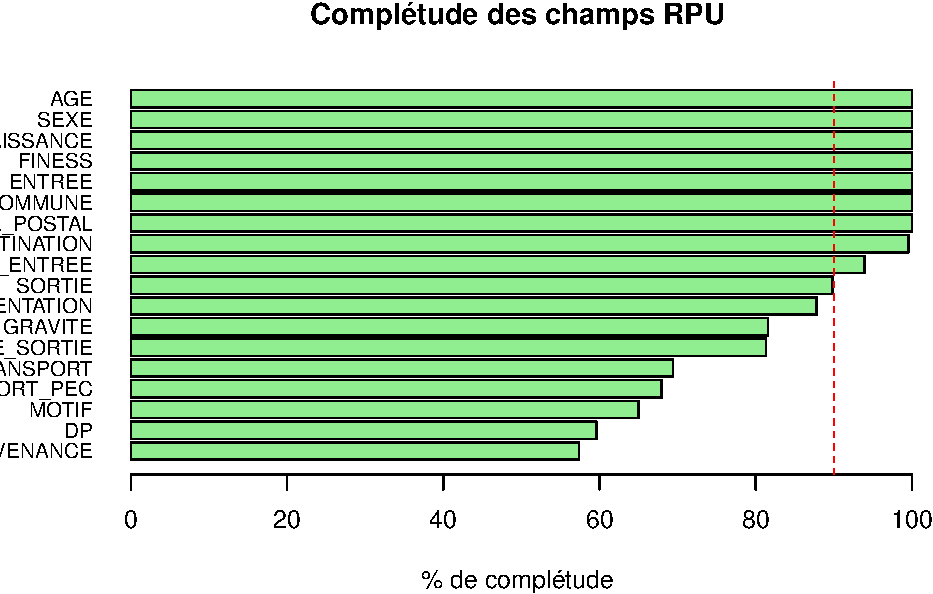
\includegraphics{rapport_2014_files/figure-latex/completude-1.pdf}
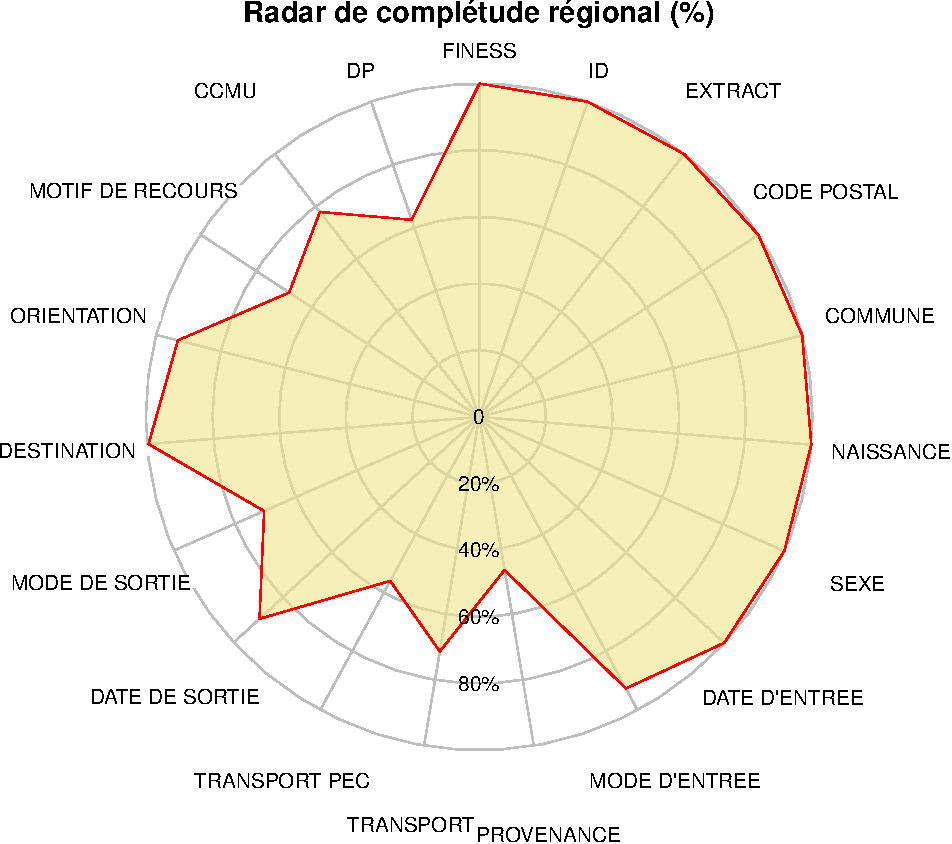
\includegraphics{rapport_2014_files/figure-latex/completude-2.pdf}

\begin{itemize}
\item
  Critères de cohérence :
\item
  \% CCMU 4 et 5 sortie externe.
\end{itemize}

\paragraph{0.12}\label{section}

\paragraph{\% de CCMU 4 et 5 renvoyé à domicile: 0.12
\%}\label{de-ccmu-4-et-5-renvoye-a-domicile-0.12}

\begin{verbatim}
- % Diagnostic hors thésaurus SFMU
- % âge > 18 ans dans SU pédiatriques.
- % diag féminin chez homme et inverse
\end{verbatim}

\begin{enumerate}
\def\labelenumi{\alph{enumi}.}
\setcounter{enumi}{3}
\itemsep1pt\parskip0pt\parsep0pt
\item
  Les travaux de la FEDORU et les travaux nationaux
\end{enumerate}

\section{le tableau récapitulatif dénommé ``Chiffres
clefs''}\label{le-tableau-recapitulatif-denomme-chiffres-clefs}

Parfois en début de rapport, parfois en fin, c'est une partie courte et
synthétique présentant, sous forme de chiffres clefs, les grands
déterminants de l'activité. Choix d'un titre commun.

\textbf{CORE {[}C{]}} obligatoire \textbf{SUPPLEMENTAL {[}S{]}}
facultatif

Analyse sur la période:

\begin{itemize}
\itemsep1pt\parskip0pt\parsep0pt
\item
  du 2015-01-01
\item
  au 2015-01-31
\item
  soit 31 jours
\end{itemize}

\subsection{Nombre de SU}\label{nombre-de-su}

(nombre de SU pédiatriques, nombre de SU polyvalents, nombre SU adultes)
{[}C{]}

\begin{itemize}
\itemsep1pt\parskip0pt\parsep0pt
\item
  Nombre de SU: 16
\end{itemize}

\subsubsection{Nombre de SU publics / privés
{[}C{]}}\label{nombre-de-su-publics-prives-c}

\begin{itemize}
\itemsep1pt\parskip0pt\parsep0pt
\item
  nombre de SU dans le secteur public: NA
\item
  nombre de SU dans le secteur privé: NA
\end{itemize}

\subsection{Nombre de passages dans l'année
{[}C{]}}\label{nombre-de-passages-dans-lannee-c}

40 509

\subsection{Moyenne quotidienne de passages
{[}C{]}}\label{moyenne-quotidienne-de-passages-c}

1 306,742

\subsection{\%(N) d'évolution par rapport à année N-1
{[}C{]}}\label{n-devolution-par-rapport-a-annee-n-1-c}

\subsection{\%(N) public/privé {[}C{]}}\label{n-publicprive-c}

\begin{itemize}
\itemsep1pt\parskip0pt\parsep0pt
\item
  nombre de RPU publics: 33936 (83.77 \%)
\item
  nombre de RPU privés: 6573 (16.23 \%)
\end{itemize}

\subsection{SEXE}\label{sexe}

\subsubsection{\%(N) Femme {[}C{]}}\label{n-femme-c}

49.39 \% (19 997)

\subsubsection{\%(N) Homme {[}C{]}}\label{n-homme-c}

50.61 \% (20 488)

\subsection{AGE}\label{age}

\subsubsection{\% (N) \textless{} 1 an {[}C{]}}\label{n-1-an-c}

1991 (4.92 \%)

\subsubsection{\%(N) \textless{} 18 ans {[}C{]}}\label{n-18-ans-c}

12769 (31.52 \%)

\subsubsection{\%(N) \textgreater{}= 75 ans {[}C{]}}\label{n-75-ans-c}

5671 (14 \%)

\subsubsection{Age moyen}\label{age-moyen}

\begin{itemize}
\item
  age moyen{[}C{]}: 37.13 ans.
\item
  age moyen des hommes {[}S{]} (pourquoi `homme et femme' en SUPP ?)
  35.34 ans.
\item
  age moyen des femmes {[}S{]} 38.99 ans.
\end{itemize}

\subsubsection{Taux de recours (définition FEDORU) régional aux
urgences.
{[}S{]}}\label{taux-de-recours-definition-fedoru-regional-aux-urgences.-s}

Utilisation des données INSEE qui collent le plus à la période d'étude
(projections ou données consolidées)

\subsubsection{\% sur activité les jours de WE
{[}S{]}}\label{sur-activite-les-jours-de-we-s}

= ((Nbsam+NbDim/2)-(sommeNbJourSEm/5))/ ((Nbsam+NbDim/2)*100
{[}Limousin{]}

6.35 \% d'activité supplémentaire le WE.

NB: le calcul ne tient pas compte des jours fériés (à faire).

\subsection{\% du delta entre mois le plus chargé et le mois le moins
chargé
{[}S{]}}\label{du-delta-entre-mois-le-plus-charge-et-le-mois-le-moins-charge-s}

100 \%

\subsection{Durées de passage}\label{durees-de-passage}

\begin{itemize}
\itemsep1pt\parskip0pt\parsep0pt
\item
  durée moyenne de passage 174.2 mn.
\item
  écart-type: 173.5035961 mn.
\item
  médiane: 123 mn.
\item
  nombre de passages \textgreater{} 4 heures: 8465 (23.61 \%).
\end{itemize}

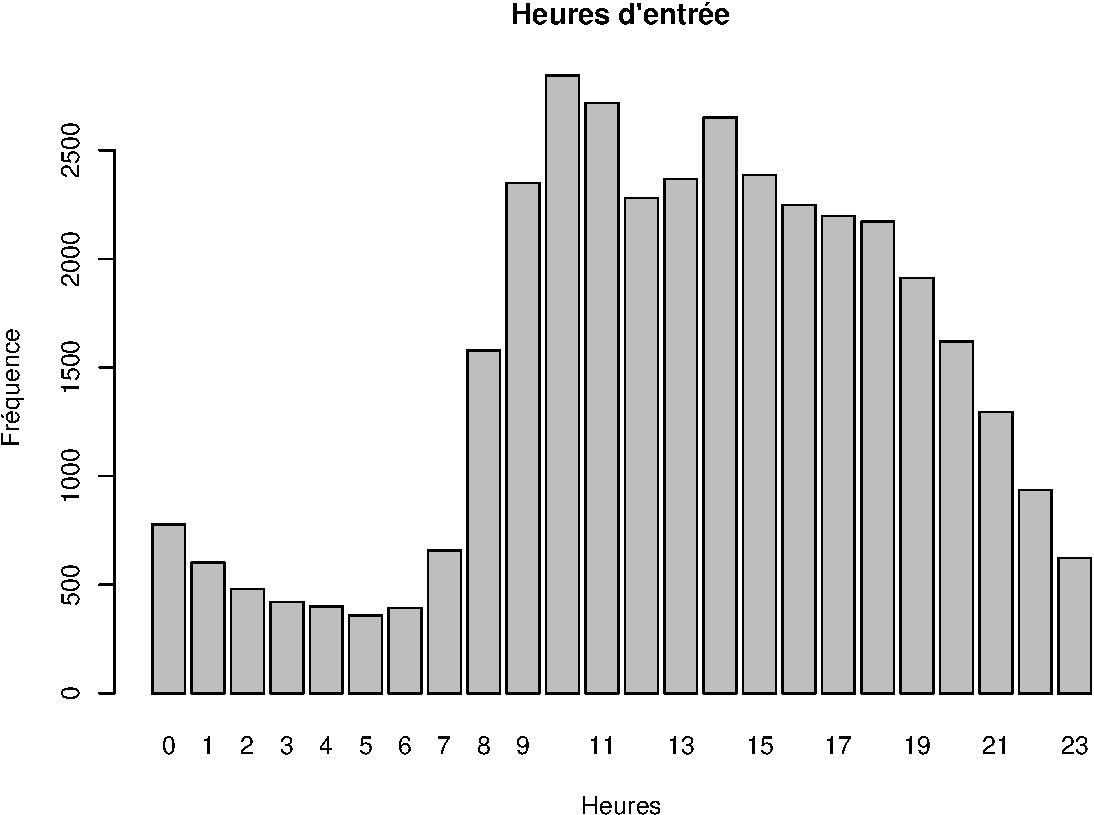
\includegraphics{rapport_2014_files/figure-latex/horaires-1.pdf}

\begin{verbatim}
##       [,1]
##  [1,]  0.7
##  [2,]  1.9
##  [3,]  3.1
##  [4,]  4.3
##  [5,]  5.5
##  [6,]  6.7
##  [7,]  7.9
##  [8,]  9.1
##  [9,] 10.3
## [10,] 11.5
## [11,] 12.7
## [12,] 13.9
## [13,] 15.1
## [14,] 16.3
## [15,] 17.5
## [16,] 18.7
## [17,] 19.9
## [18,] 21.1
## [19,] 22.3
## [20,] 23.5
## [21,] 24.7
## [22,] 25.9
## [23,] 27.1
## [24,] 28.3
\end{verbatim}

\subsubsection{\% passages nuit (définition FEDORU)
{[}C{]}}\label{passages-nuit-definition-fedoru-c}

nombre de passages dont l'admission s'est effectuée sur la période
{[}20h00 - 7h59{]} divisé par l'ensemble des passages

23.61 \% (N = 8561)

\subsubsection{\% passages nuit profonde (définition FEDORU)
{[}C{]}}\label{passages-nuit-profonde-definition-fedoru-c}

nombre de passages dont l'admission s'est effectuée sur la période
{[}00h00 - 7h59{]} divisé par l'ensemble des passages

11.27 \% (N = 4088)

\subsection{Mode de transport}\label{mode-de-transport}

\subsubsection{\%(N) d'arrivée perso {[}S{]}}\label{n-darrivee-perso-s}

68.91 \% (N = 19 913)

\subsubsection{\%(N) d'arrivée SMUR {[}S{]}}\label{n-darrivee-smur-s}

1.06 \% (N = 305)

\subsubsection{\%(N) d'arrivée VSAB {[}S{]}}\label{n-darrivee-vsab-s}

10.3 \% (N = 2 977)

\subsubsection{\%(N) d'arrivée Ambulance
{[}S{]}}\label{n-darrivee-ambulance-s}

19.13 \% (N = 5 527)

\subsection{Gravité (CCMU)}\label{gravite-ccmu}

\subsubsection{\%(N) CCMU 1 et 2 {[}C{]}}\label{n-ccmu-1-et-2-c}

84.16\% (n = 26549)

\subsubsection{\%(N) CCMU 4 et 5 {[}C{]}}\label{n-ccmu-4-et-5-c}

1.38\% (n = 434)

\subsubsection{\%(N) Médico-chir {[}C{]}}\label{n-medico-chir-c}

\subsubsection{\%(N) Traumato {[}C{]}}\label{n-traumato-c}

\subsubsection{\%(N) Psy {[}C{]}}\label{n-psy-c}

0.39\% (n = 124)

\subsection{Durée de présence}\label{duree-de-presence}

\subsubsection{Durée de séjour (hors
UHCD):}\label{duree-de-sejour-hors-uhcd}

moyenne +/- ET ; médiane (IQR) {[}C{]}

\begin{itemize}
\itemsep1pt\parskip0pt\parsep0pt
\item
  moyenne: 174.2 mn
\item
  écart-type: 173.5035961 mn
\item
  médiane: 123 mn
\item
  IQR: 169 mn
\end{itemize}

\subsubsection{\% (N) passages ayant durée attente \textgreater{} 1
heure {[}S{]}}\label{n-passages-ayant-duree-attente-1-heure-s}

Pas calculable en Alsace :-(

\subsubsection{\% (N) passages durée séjour \textgreater{} 4h
{[}S{]}}\label{n-passages-duree-sejour-4h-s}

23.61\% (n = 8465)

\subsection{Mode de sortie}\label{mode-de-sortie}

\subsubsection{\% (N)Externe {[}C{]}}\label{nexterne-c}

75.36 \% (N = 21 497)

\subsubsection{\% (N)Hospitalisation {[}C{]}}\label{nhospitalisation-c}

23.1 \% (N = 6 590)

\subsubsection{\% (N)Transfert {[}C{]}}\label{ntransfert-c}

1.54 \% (N = 439)

\subsubsection{\% (N)Sortie non convenue
{[}C{]}}\label{nsortie-non-convenue-c}

4.58 \% (N = 336)

\subsubsection{\% (N)Décès {[}C{]}}\label{ndeces-c}

0\% (n = 1)

\section{les résultats régionaux}\label{les-resultats-regionaux}

partie centrale du rapport dans laquelle tous les résultats d'activité
sont présentés dans le déroulement d'une trame. Le principe est de
passer en revue les variables du RPU (communes à tous normalement), d'en
proposer une exploitation si elles présentent un intérêt, puis de
proposer quelques croisements associés à chaque variable s'ils semblent
pertinents (présence d'un bloc `croisement' spécifique dans chaque
partie ci dessous).

\subsection{Volume global d'activité, cumul de
passages}\label{volume-global-dactivite-cumul-de-passages}

\paragraph{historique du nombre de
passages}\label{historique-du-nombre-de-passages}

\paragraph{{[}1{]}{[}2{]} par année et de la moyenne quotidienne du
nombre de
passages}\label{par-annee-et-de-la-moyenne-quotidienne-du-nombre-de-passages}

Graphe avec 2 axes des abcisses:

\begin{itemize}
\itemsep1pt\parskip0pt\parsep0pt
\item
  total par année
\item
  moyenne quotidienne par année
\end{itemize}

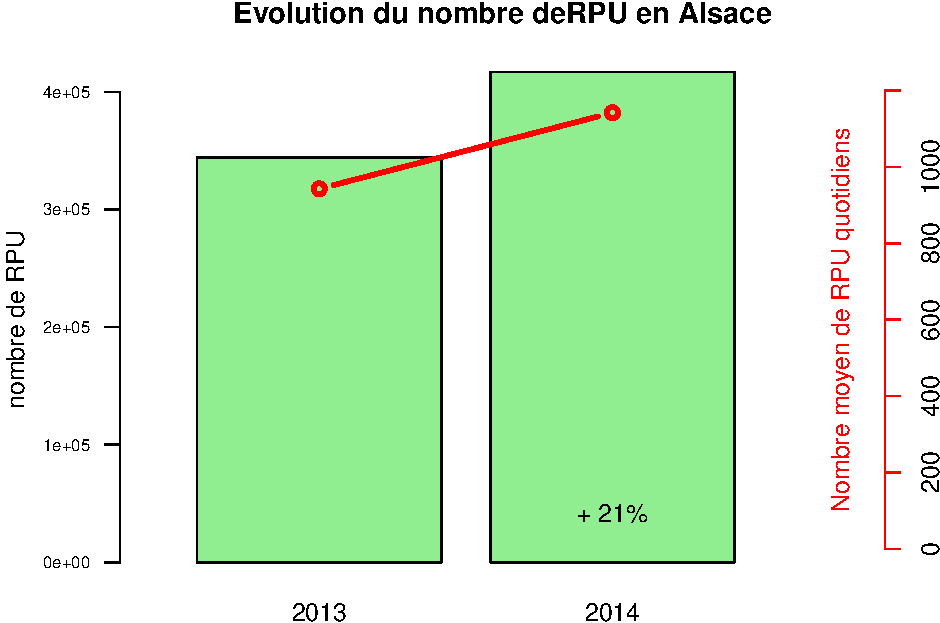
\includegraphics{rapport_2014_files/figure-latex/c1-1.pdf}

\begin{itemize}
\itemsep1pt\parskip0pt\parsep0pt
\item
  nombre de passages en 2014: 40 509 soit en moyenne 111 par jour.
\end{itemize}

\paragraph{{[}3{]} \% d'augmentation annuelle sur les années
disponibles}\label{daugmentation-annuelle-sur-les-annees-disponibles}

\% de variation 2014/2013 = -88.23 \%

croisements :

\paragraph{{[}4{]}{[}5{]} nombre de passages et \% par type de
structures (CH, CHU, privé), année
N}\label{nombre-de-passages-et-par-type-de-structures-ch-chu-prive-annee-n}

On utilise le fichier \textbf{Hopitaux\_Alsace2.csv} qui comporte les
informations suivantes:

\begin{itemize}
\itemsep1pt\parskip0pt\parsep0pt
\item
  nom de la structure
\item
  aabréviation pour lesRPU
\item
  FINESS géographique
\item
  FINESS juridique
\item
  Groupe juridique (ex. GHSV)
\item
  Territoire de santé
\item
  Zone de proximité
\item
  type
\item
  statut
\item
  nombre total de lits
\item
  nombre de lits de chirurgie
\item
  nombre de lits de médecine
\end{itemize}

Le calcul se fait après un merging de dx et de hop.

\begin{verbatim}
     2014        %          
CH   "24 746.00" "    61.09"
CHU  " 9 190.00" "    22.69"
PSPH " 6 573.00" "    16.23"
     "40 509.00" "   100.01"
\end{verbatim}

\paragraph{{[}6{]} \% CH, CHU, privé sur les années
disponibles}\label{ch-chu-prive-sur-les-annees-disponibles}

\subsection{Caractéristique des patients :
âge}\label{caracteristique-des-patients-age}

\begin{itemize}
\itemsep1pt\parskip0pt\parsep0pt
\item
  {[}7{]}{[}8{]} moyenne âge +/- écart type année N
\end{itemize}

moyenne d'age: 37.129925 ans, ecart-type: 27.8`ans.

\begin{itemize}
\itemsep1pt\parskip0pt\parsep0pt
\item
  {[}9{]} répartition par tranche âge
\end{itemize}

\begin{verbatim}
[1] "ToDo"
\end{verbatim}

\begin{verbatim}
a
    [0,5)    [5,10)   [10,15)   [15,20)   [20,25)   [25,30)   [30,35) 
     5965      2460      2759      2617      2515      2490      2211 
  [35,40)   [40,45)   [45,50)   [50,55)   [55,60)   [60,65)   [65,70) 
     1929      2003      1924      1869      1736      1584      1440 
  [70,75)   [75,80)   [80,85)   [85,90)   [90,95)  [95,100) [100,105) 
     1335      1482      1763      1456       809       138        20 
[105,110) [110,115) [115,120] 
        0         3         0 
\end{verbatim}

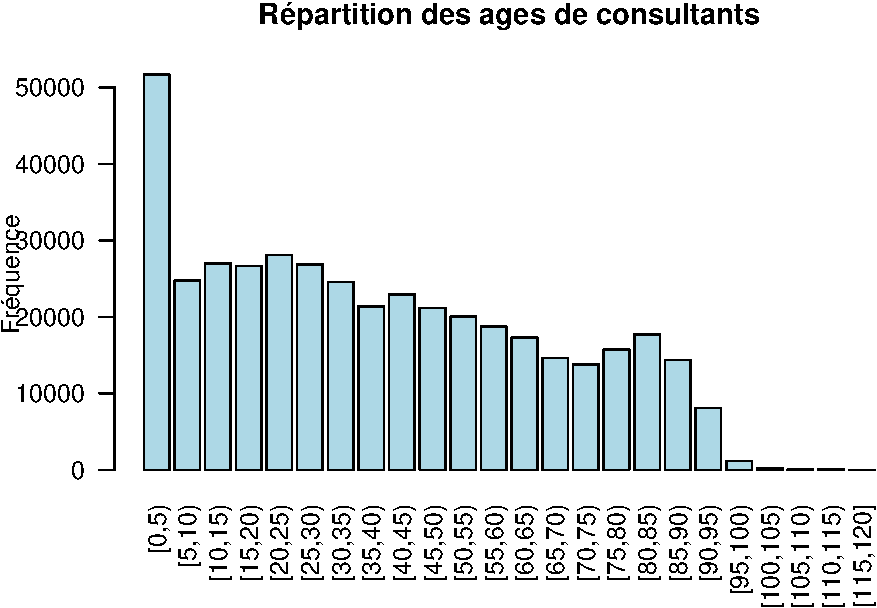
\includegraphics{rapport_2014_files/figure-latex/tranche-1.pdf}

\begin{itemize}
\itemsep1pt\parskip0pt\parsep0pt
\item
  {[}10{]} pyramide des âges des patients accueillis aux urgences année
  N
\end{itemize}

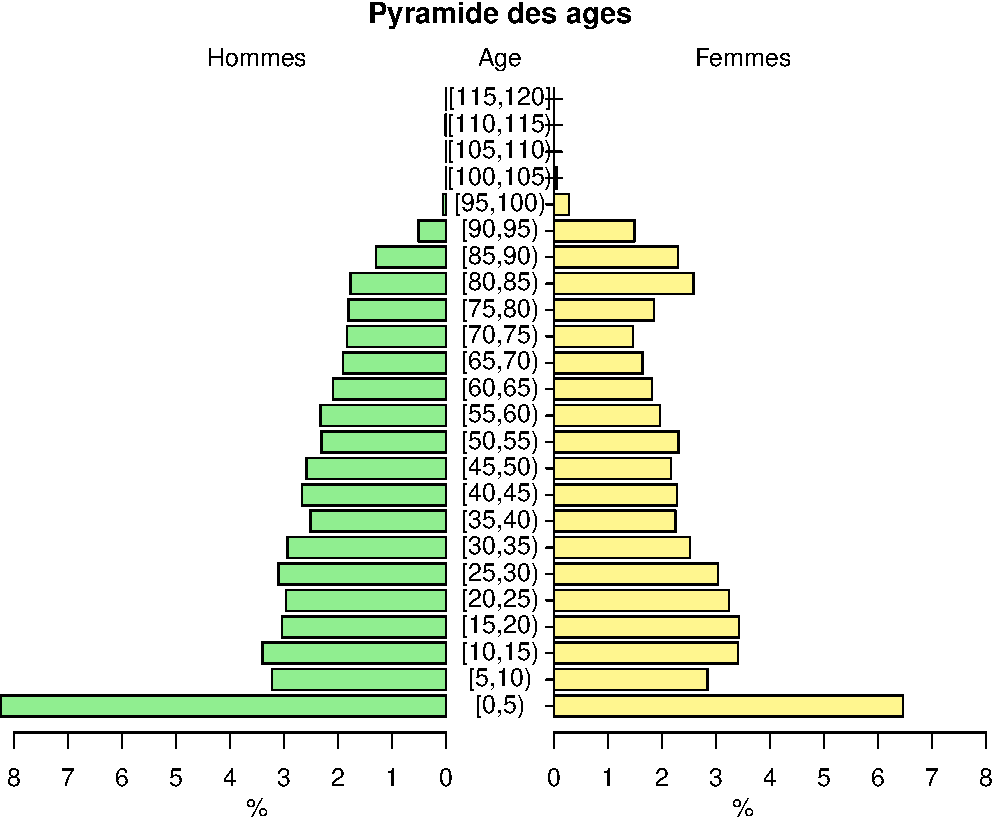
\includegraphics{rapport_2014_files/figure-latex/pyramide-1.pdf}

\begin{verbatim}
## [1] 5.1 4.1 4.1 2.1
\end{verbatim}

\begin{itemize}
\item
  croisements :
\item
  {[}11{]} sexe-moyenne âge femme/homme, année N
\end{itemize}

\begin{verbatim}
##        F        I        M 
## 38.99030 16.41667 35.33831
\end{verbatim}

\begin{itemize}
\itemsep1pt\parskip0pt\parsep0pt
\item
  {[}12{]} proportion des âge extrêmes (moins de 1 an, plus de 90 ans)
  par mois, année N
\end{itemize}

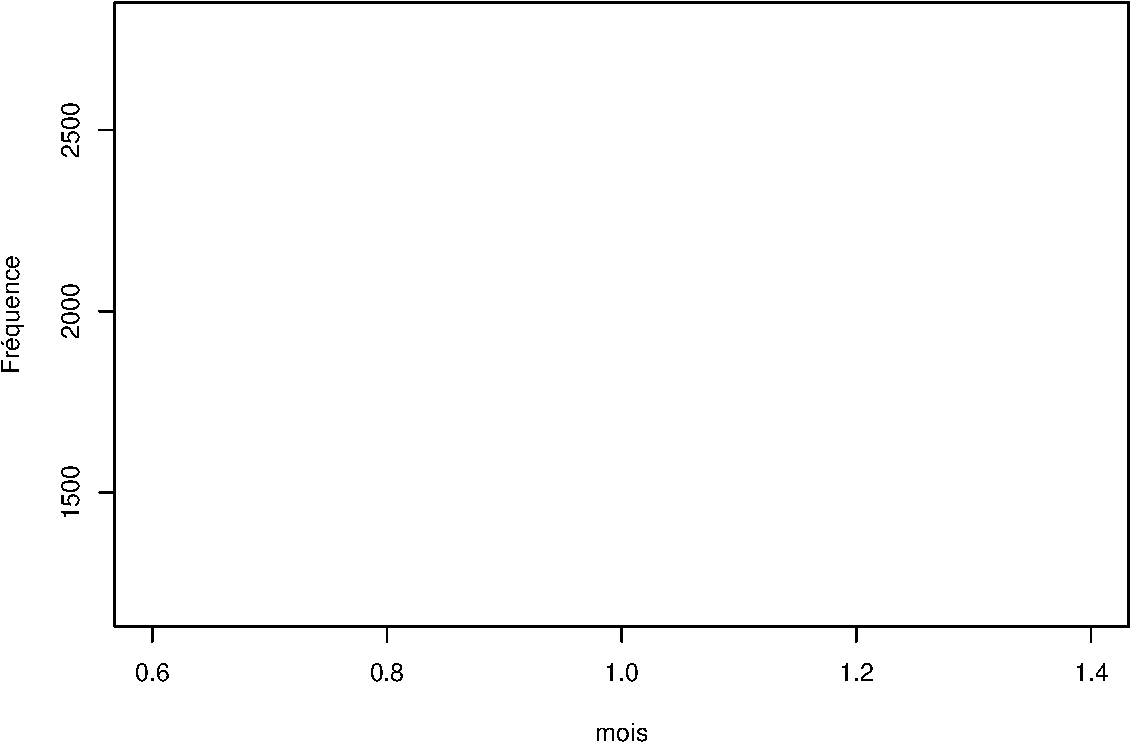
\includegraphics{rapport_2014_files/figure-latex/age_extreme-1.pdf}
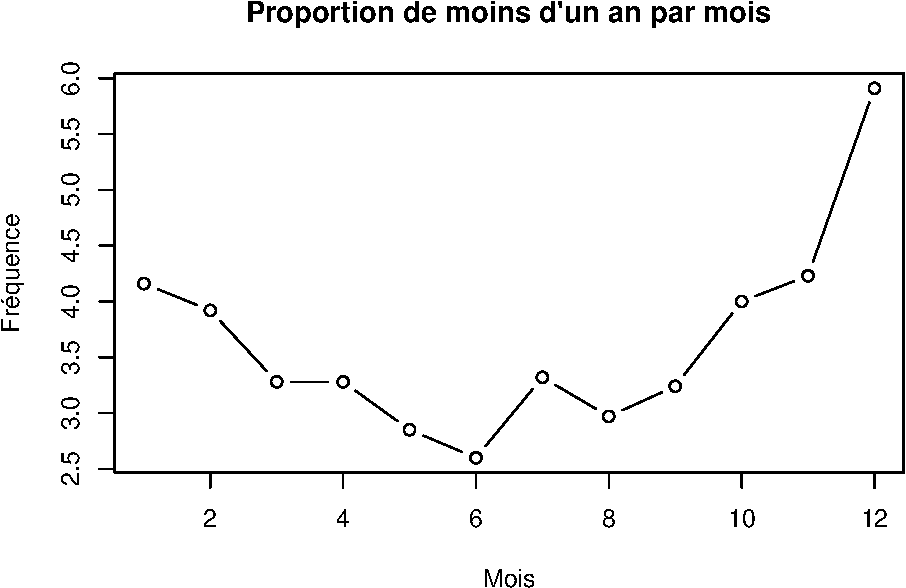
\includegraphics{rapport_2014_files/figure-latex/age_extreme-2.pdf}
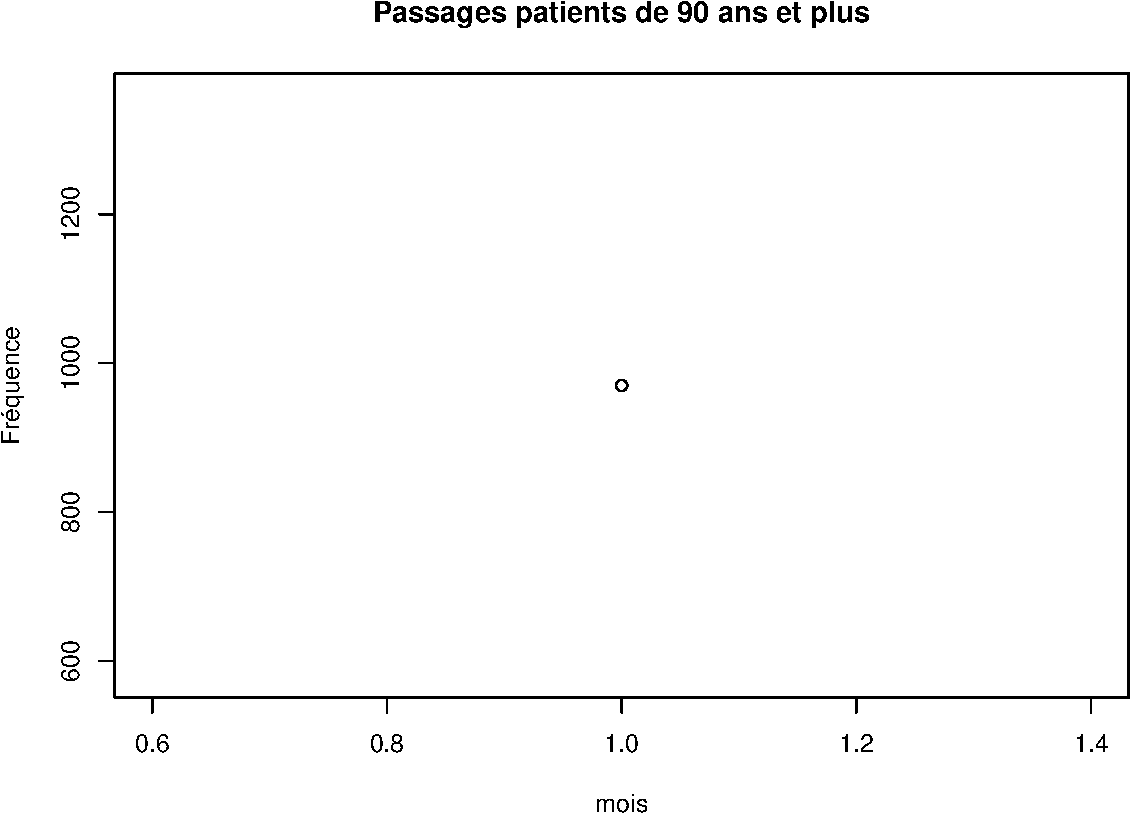
\includegraphics{rapport_2014_files/figure-latex/age_extreme-3.pdf}
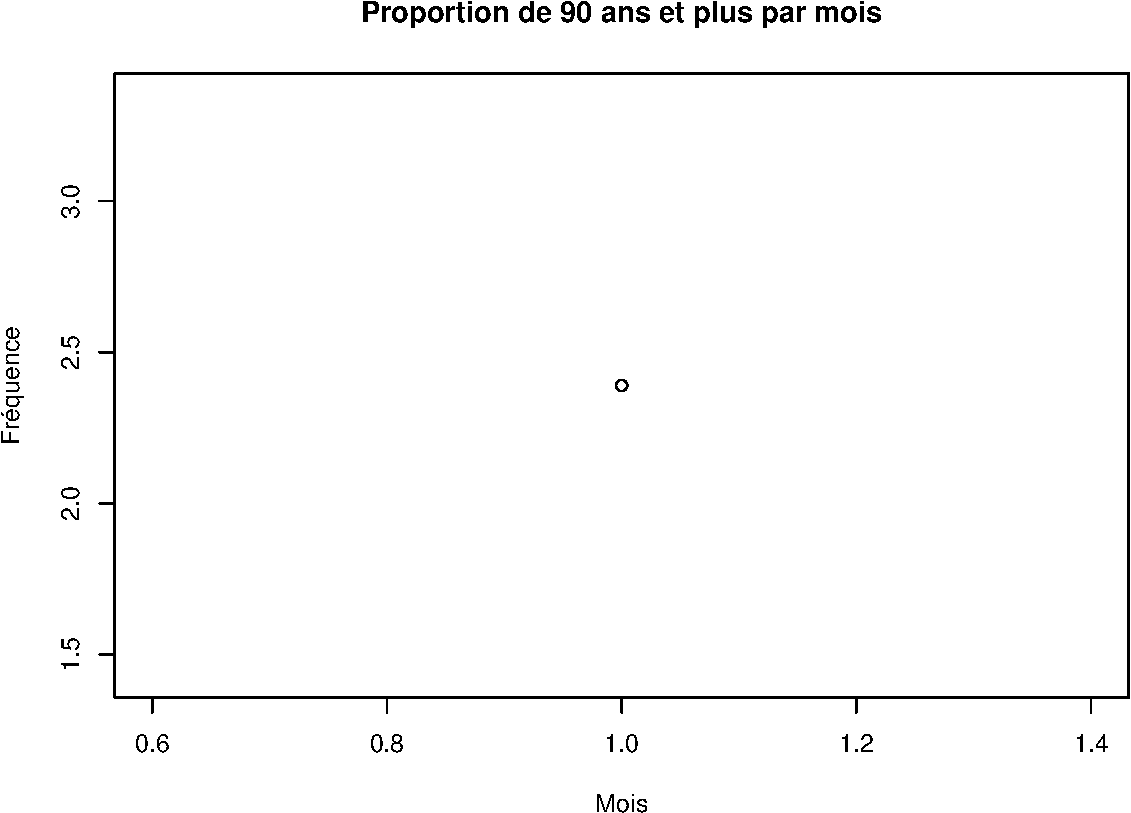
\includegraphics{rapport_2014_files/figure-latex/age_extreme-4.pdf}

\subsection{Caractéristique des patients :
sexe}\label{caracteristique-des-patients-sexe}

\begin{itemize}
\itemsep1pt\parskip0pt\parsep0pt
\item
  {[}13{]} répartition en fonction du sexe année N
\end{itemize}

\begin{verbatim}
## 
##     F     I     M 
## 19997    24 20488
\end{verbatim}

\begin{itemize}
\itemsep1pt\parskip0pt\parsep0pt
\item
  {[}14{]} sex ratio, année N
\end{itemize}

sex-ratio = 1.0245537

\begin{itemize}
\item
  croisements :
\item
  {[}15{]} sex ratio H/F par classe d'âge, année N
\end{itemize}

\begin{verbatim}
##      [0,5)     [5,10)    [10,15)    [15,20)    [20,25)    [25,30) 
## 1.27588842 1.13194444 0.99927484 0.88544669 0.91539634 1.02276423 
##    [30,35)    [35,40)    [40,45)    [45,50)    [50,55)    [55,60) 
## 1.16568627 1.11868132 1.16774892 1.19134396 1.00000000 1.18090452 
##    [60,65)    [65,70)    [70,75)    [75,80)    [80,85)    [85,90) 
## 1.15217391 1.16216216 1.25126476 0.97600000 0.68546845 0.56620022 
##    [90,95)   [95,100)  [100,105)  [105,110)  [110,115)  [115,120] 
## 0.34162521 0.21052632 0.05263158         NA 2.00000000         NA
\end{verbatim}

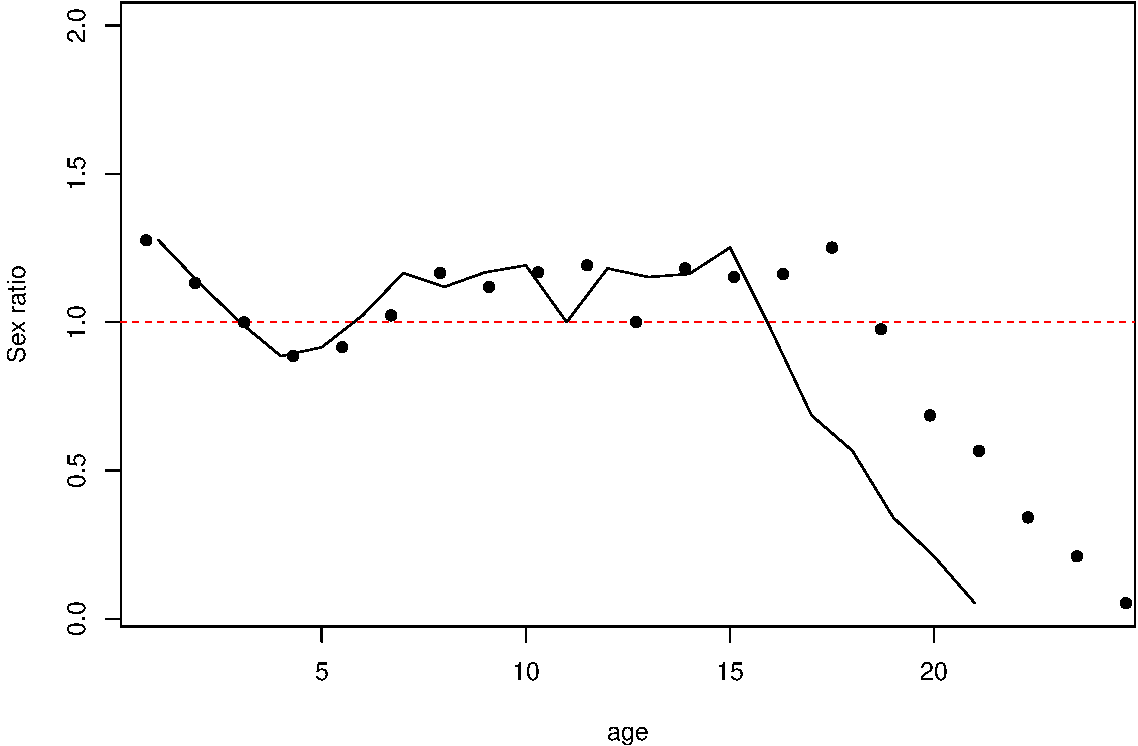
\includegraphics{rapport_2014_files/figure-latex/ratio_classe_age-1.pdf}

\begin{itemize}
\itemsep1pt\parskip0pt\parsep0pt
\item
  {[}16{]} taux de masculinité
\end{itemize}

0.51

\subsection{Provenance géographique des
patients}\label{provenance-geographique-des-patients}

\begin{itemize}
\item
  population régionale (INSEE)
\item
  provenance région / hors région / étranger, année N
\item
  cartographie des pourcentages d'activité que représentent les passages
  de patients provenant des départements limitrophes, année N
\item
  cartographie du nombre de passages régional en fonction du lieu de
  résidence du patient (code postal) année N
\item
  pourcentage de patient ne résidant pas dans une zone postale où est
  installée une structure d'urgence, année N
\end{itemize}

croisements :

\begin{itemize}
\itemsep1pt\parskip0pt\parsep0pt
\item
  cartographie des taux de recours année N
\item
  taux de recours / âge et / sexe, année N
\item
  évolution par mois des moyennes quotidiennes de passages des
  populations région / hors région / étranger, année N
\end{itemize}

\subsection{Arrivée aux urgences}\label{arrivee-aux-urgences}

\begin{itemize}
\item
  Moyenne quotidienne du nombre de passages par mois (basée sur la date
  d'admission) année N
  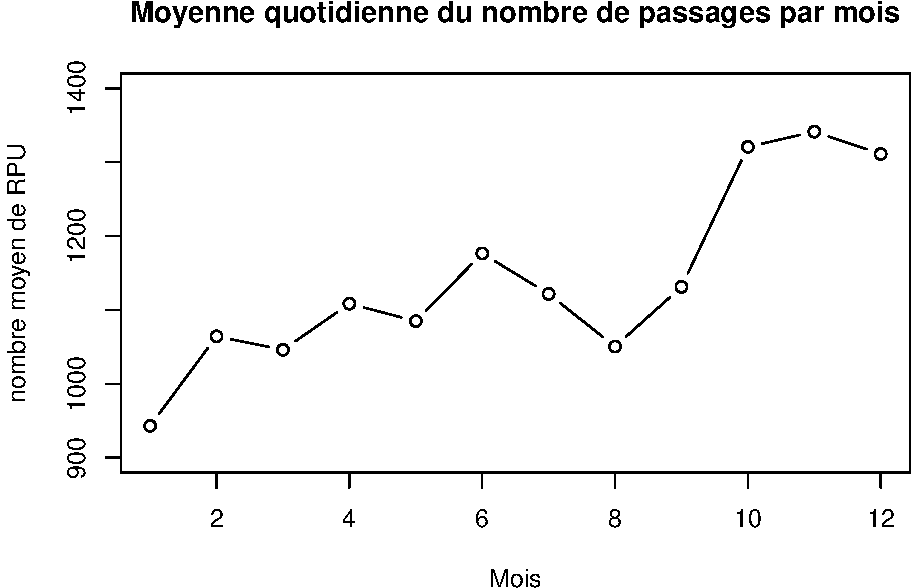
\includegraphics{rapport_2014_files/figure-latex/mean_month-1.pdf}
\item
  Nombre de passages par semaine (basée sur la date d'admission) année N
  (positionner les vacances scolaires de la zone concernée)
  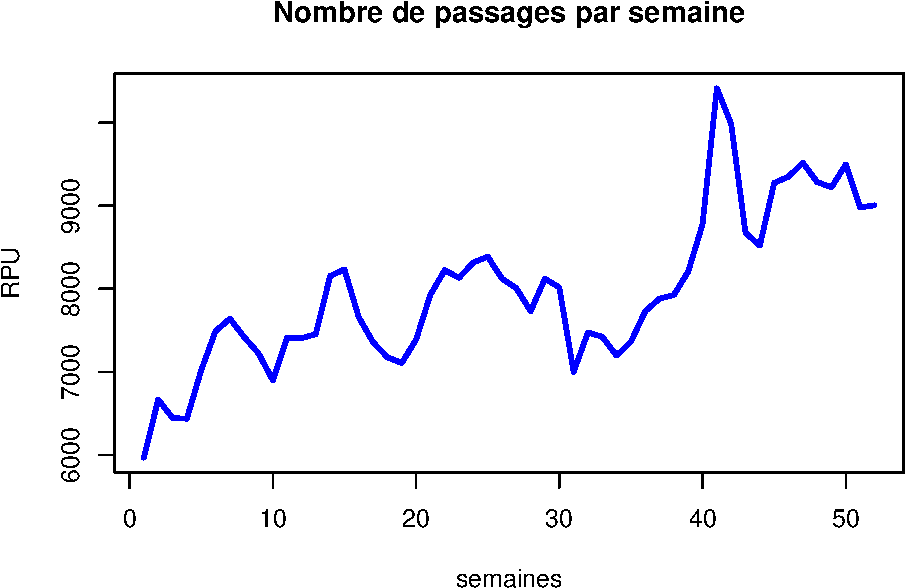
\includegraphics{rapport_2014_files/figure-latex/rpu_semaine-1.pdf}
\item
  Moyenne quotidienne du nombre de passages par jour de semaine (basée
  sur la date d'admission), année N
\item
  Répartition semaine/week-end (basée sur la date d'admission), année N
\item
  Moyenne quotidienne du nombre de passages par « tranche d'heure »
  d'entrée , année N
\item
  Pourcentage du nombre de passages par heure d'entrée et de sortie,
  année N
\item
  Répartition jour/nuit (\%), année N
\item
  Nombre de passages et \% réalisés durant les horaires PDS
\end{itemize}

croisements :

\begin{itemize}
\itemsep1pt\parskip0pt\parsep0pt
\item
  Différentiel d'activité en \% été/hiver (pourcentage de variation du
  nombre de passages entre l'été (ou l'hiver) et le reste de l'année)
  par - - type de SU (adulte, pédia, polyvalent)
\item
  \% de catégorie d'âge (pédia, âge moyen, géria) en fonction de la
  tranche d'heure d'entrée, année N
\item
  \% de classe d'âge (pédia, âge moyen, géria) en fonction de l'heure
  d'entrée, année N
\item
  Taux d'hospitalisation et taux de retour à domicile en fonction de
  l'heure d'entrée, année N
\item
  \% du type de recours (trauma, psy, medico chir) en fonction de
  l'heure d'entrée, année N
\item
  \% du mode de transport à l'entrée (VSAV, SMUR, AP,\ldots{}) en
  fonction de l'heure d'entrée, année N
\item
  Moyenne quotidienne du nombre de passages par semaine, (basée sur la
  date d'admission) en fonction du type de SU (polyvalent, pédia,
  adulte), année N
\end{itemize}

\subsection{Mode de transport à l'arrivée aux
urgences}\label{mode-de-transport-a-larrivee-aux-urgences}

\begin{itemize}
\itemsep1pt\parskip0pt\parsep0pt
\item
  Répartition des modes de transport (à l'arrivée aux urgences), année
  N, évolution
\end{itemize}

croisements :

\begin{itemize}
\itemsep1pt\parskip0pt\parsep0pt
\item
  Mode de transport (à l'arrivée aux urgences) par département
\item
  Mode de transport (à l'arrivée aux urgences) par type de structure
  (CH, CHU, privé)
\item
  Mode de transport (à l'arrivée aux urgences) par tranche d'âge
\item
  Mode de transport (à l'arrivée aux urgences) par CCMU regroupé
  ({[}1;2{]} ; 3 ; {[}4;5{]})
\end{itemize}

\subsection{Gravité}\label{gravite}

\begin{itemize}
\itemsep1pt\parskip0pt\parsep0pt
\item
  répartition CCMU par regroupement ({[}1;2{]} ; 3 ; {[}4;5{]}; D; P),
  année N
\end{itemize}

croisements :

\begin{itemize}
\itemsep1pt\parskip0pt\parsep0pt
\item
  pourcentage de CCMU 1 et 2 par tranche d'âge, année N
\item
  pourcentage de CCMU 4 et 5 par tranche d'âge, année N
\end{itemize}

\subsection{Motif de recours}\label{motif-de-recours}

\begin{verbatim}
- Nombre de passages par motif, année N 
\end{verbatim}

\subsection{Pathologie}\label{pathologie}

\begin{itemize}
\itemsep1pt\parskip0pt\parsep0pt
\item
  répartition par type d'urgences (med/chir, traumato, psy, toxico,
  autre), année N
\item
  répartition par entêtes chapitre CIM 10, année N
\item
  répartition par disciplines, année N
\item
  répartition par diagnostic principal (top 10), année N
\item
  répartition par diagnostic principal (top 5) en fonction du type
  d'urgences (med/chir, traumato, psy, toxico, autre), année N
\end{itemize}

croisements :

\begin{verbatim}
- Type d’urgences (med/chir, traumato, psy, toxico, autre) en fonction de la classe d’âge (pédia, âge moyen, géria), année N
\end{verbatim}

\begin{itemize}
\itemsep1pt\parskip0pt\parsep0pt
\item
  TOP 10 diagnostic principal en fonction du sexe, année N
\end{itemize}

\subsection{Temps de passage}\label{temps-de-passage}

\begin{itemize}
\itemsep1pt\parskip0pt\parsep0pt
\item
  Temps de passage moyen +/- ET et médian (IQR), année N
\item
  Répartition des passages par durée de passage en classe
\item
  Pourcentage cumulé des temps de passage, année N
\end{itemize}

Croisements :

\begin{verbatim}
- Temps de passage médian en fonction de la classe d’âge (pédia, âge moyen, géria), année N
\end{verbatim}

\begin{itemize}
\itemsep1pt\parskip0pt\parsep0pt
\item
  Temps de passage médian par type de structure (CH, CHU, privé), année
  N
\item
  Temps de passage médian par type de SU (polyvalent / ped/ adulte),
  année N
\item
  Temps de passage médian selon catégories de nombre de passage annuel
  dans les SU, année N
\item
  Temps de passage médian en fonction du mode d'entrée année N
\item
  Temps de passage médian en fonction de CCMU (CCMU1, CCMU4\&5), année N
\item
  Temps de passage médian en fonction du sexe, année N
\item
  Temps de passage médian en fonction du type d'urgences (med/chir,
  traumato, psy, toxico, autre), année N
\item
  TOP 10 diagnostic principal pour lequel le temps de passage médian est
  le plus long / le plus court, année N
\item
  Temps de passage médian en fonction de l'orientation du patient, année
  N
\item
  Temps de passage médian en fonction de l'heure d'entrée et de l'heure
  de sortie, année N
\end{itemize}

\subsection{Orientation}\label{orientation}

\begin{itemize}
\itemsep1pt\parskip0pt\parsep0pt
\item
  Moyenne quotidienne du nombre de passages en fonction de
  l'orientation, année N
\end{itemize}

\begin{verbatim}
##      CHIR     FUGUE       HDT        HO       MED      OBST       PSA 
## 41.516129  1.250000  1.153846  1.000000 83.387097  1.363636  9.322581 
##       REA       REO        SC      SCAM        SI      UHCD 
##  5.516129  4.333333  7.387097  1.684211 12.290323 70.354839
\end{verbatim}

\begin{verbatim}
##  CHIR FUGUE   HDT    HO   MED  OBST   PSA   REA   REO    SC  SCAM    SI 
##  1287    15    15     3  2585    15   289   171   130   229    32   381 
##  UHCD 
##  2181
\end{verbatim}

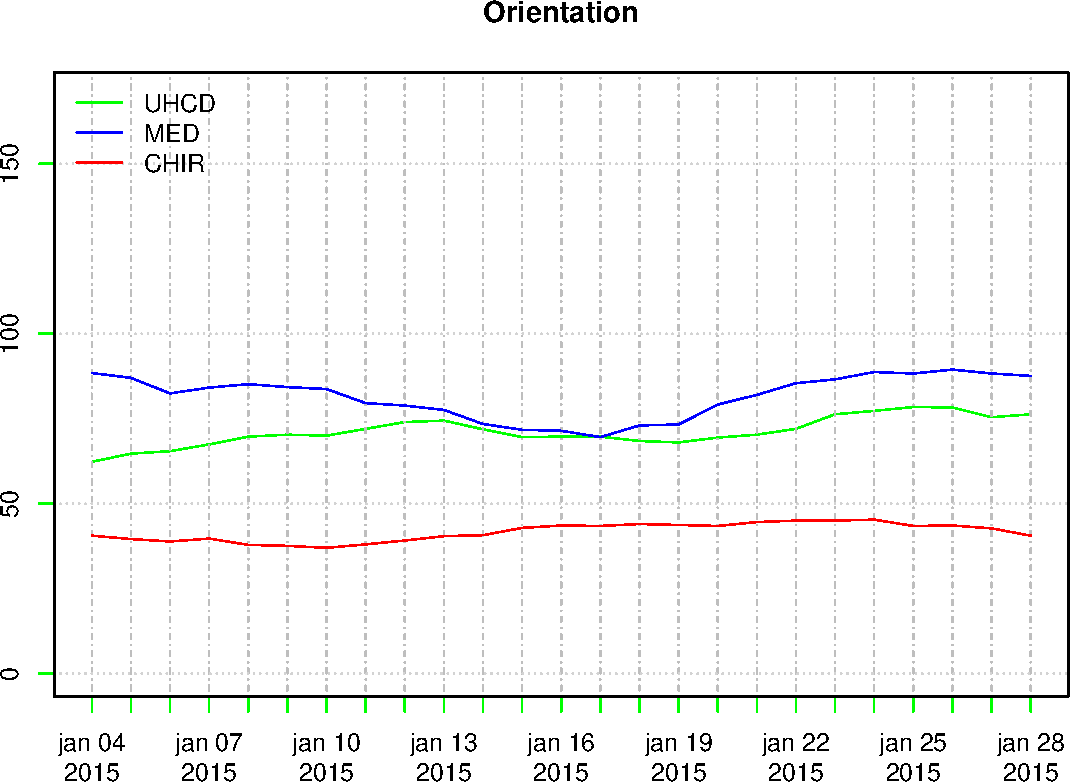
\includegraphics{rapport_2014_files/figure-latex/moyenne-orientation-1.pdf}

croisements :

\begin{itemize}
\itemsep1pt\parskip0pt\parsep0pt
\item
  Moyenne quotidienne du nombre d'hospitalisations en fonction de la
  classe d'âge (pédia, âge moyen, géria), année N
\item
  Taux d'hospitalisation en fonction de jour/nuit et âge, année N
\item
  Top 5 des disciplines pathologiques pour lesquelles le taux
  d'hospitalisation est le plus fort, année N
\item
  Top 5 des disciplines pathologiques pour lesquelles le taux de retour
  à domicile est le plus fort, année N
\item
  Cartographie du taux de retour à domicile en fonction du lieu de
  résidence du patient (code postal) année N
\item
  Nombre de décès par semaine, année N
\end{itemize}

\subsection{les analyses par filière}\label{les-analyses-par-filiere}

focus sur une sous déclinaison de l'activité (pathologies traceuses ou
traits caractéristiques de la patientèle)

\paragraph{AVC : (définition FEDORU)}\label{avc-definition-fedoru}

\begin{itemize}
\itemsep1pt\parskip0pt\parsep0pt
\item
  Nombre de passages AVC urgences, année N
\item
  Nombre de passages AVC urgences, déclinaison par département,
  établissement, année N
\item
  Moyenne quotidienne, année N
\item
  Age moyen, année N
\item
  Répartition par classe âge en pourcentage, année N
\item
  Répartition par sexe en pourcentage, année N
\item
  TOP 5 pourcentage par code CIM 10, année N
\item
  Répartition we/semaine en pourcentage, année N
\item
  Répartition par tranche heure en pourcentage, année N
\item
  Répartition par orientation en pourcentage, année N
\item
  Temps de passage médian, année N
\end{itemize}

\section{Définitions FEDORU}\label{definitions-fedoru}

\subsection{taux de recours (de la région ou
département)}\label{taux-de-recours-de-la-region-ou-departement}

nombre de passages dans les services d'urgences (de la région ou
département) de patients résidant dans une zone donnée (code postal ou
commune) divisé par la population estimée de cette zone sur la période
donnée.

\subsection{pourcentage de passage
nuit}\label{pourcentage-de-passage-nuit}

nombre de passages dont l'admission s'est effectuée sur la période
{[}20h00 - 7h59{]} divisé par l'ensemble des passages

\subsection{pourcentage de passage nuit
profonde}\label{pourcentage-de-passage-nuit-profonde}

nombre de passages dont l'admission s'est effectuée sur la période
{[}00h00 - 7h59{]} divisé par l'ensemble des passages

\subsection{tranche d'âge}\label{tranche-dage}

\begin{verbatim}
<28j;[28j-1A[;[1-5[;[5-10[;[10-15[;[15-18[;[18-30[;[30-45[;[45;65[;[65-75[;[75;85[;>85ans
\end{verbatim}

\subsection{sexe}\label{sexe-1}

M/F/I

\subsection{« tranche d'heure » d'entrée}\label{tranche-dheure-dentree}

matinée {[}8h00-11h59{]} ; début d'après midi {[}12h00-15h59{]} ; fin
d'après midi {[}16h00-19h59{]} ; soirée {[}20h00-23h59{]} ; nuit
profonde {[}00h00;07h59{]}
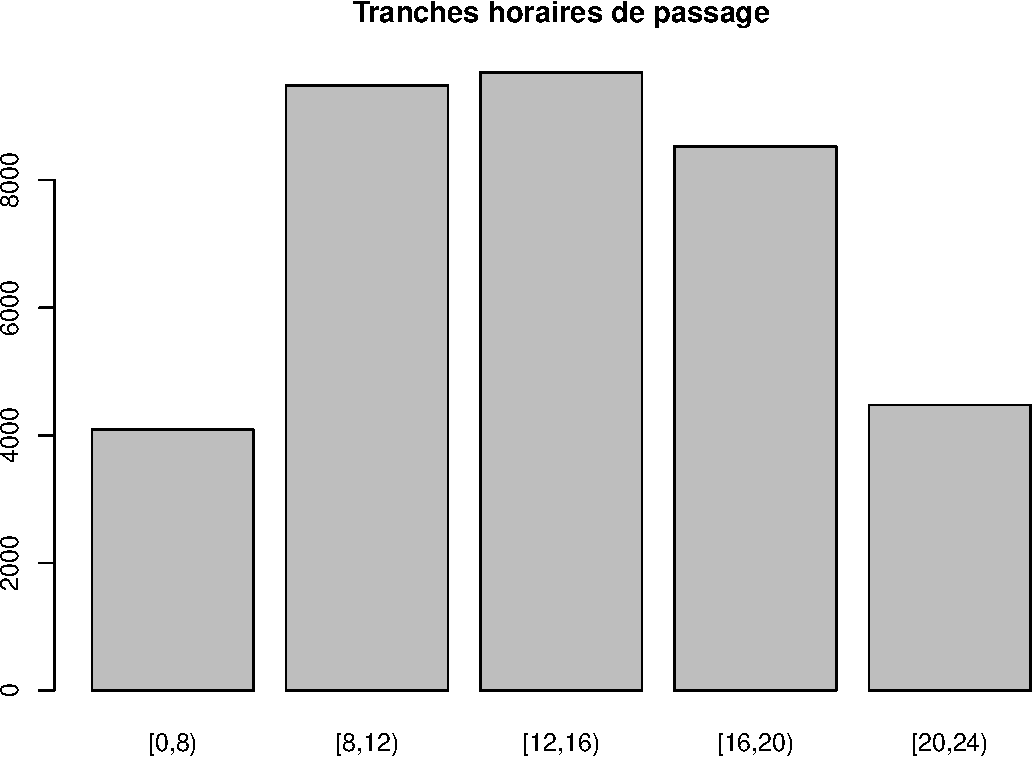
\includegraphics{rapport_2014_files/figure-latex/tranches_heure_entree-1.pdf}

\subsection{horaire PDS}\label{horaire-pds}

\begin{itemize}
\itemsep1pt\parskip0pt\parsep0pt
\item
  week end PDSA: du samedi 12h00 au lundi 07h59
\item
  en semaine: du lundi au vendredi de {[}20h00 - 07h59{]} le lendemain
\item
  jour férié: de 00h00 à 23h59
\item
  pont PDSA: de 00h00 à 23h59
\end{itemize}

Les ponts PDSA sont ceux qui sont qualifiés comme tel par l'ARS et qui
génère à ce titre le mise en place d'une régulation PDSA sur cette
période. Si un pont PDSA, ou un jour férié survient un vendredi, le
samedi matin suivant sera dès lors intégré à l'activité PDSA.

\subsection{durée de passage en
classe}\label{duree-de-passage-en-classe}

2 types de regroupements :

\begin{itemize}
\itemsep1pt\parskip0pt\parsep0pt
\item
  moins de 4 heures ; 4 heures et plus
\item
  moins d'une heure ; entre 1 et 2 heures ; de 2 à 4 heures ; de 4 à 8
  heures ; de 8 à 12 heures ; entre 12 et 72 heures ; (bornes
  supérieures exclues)
  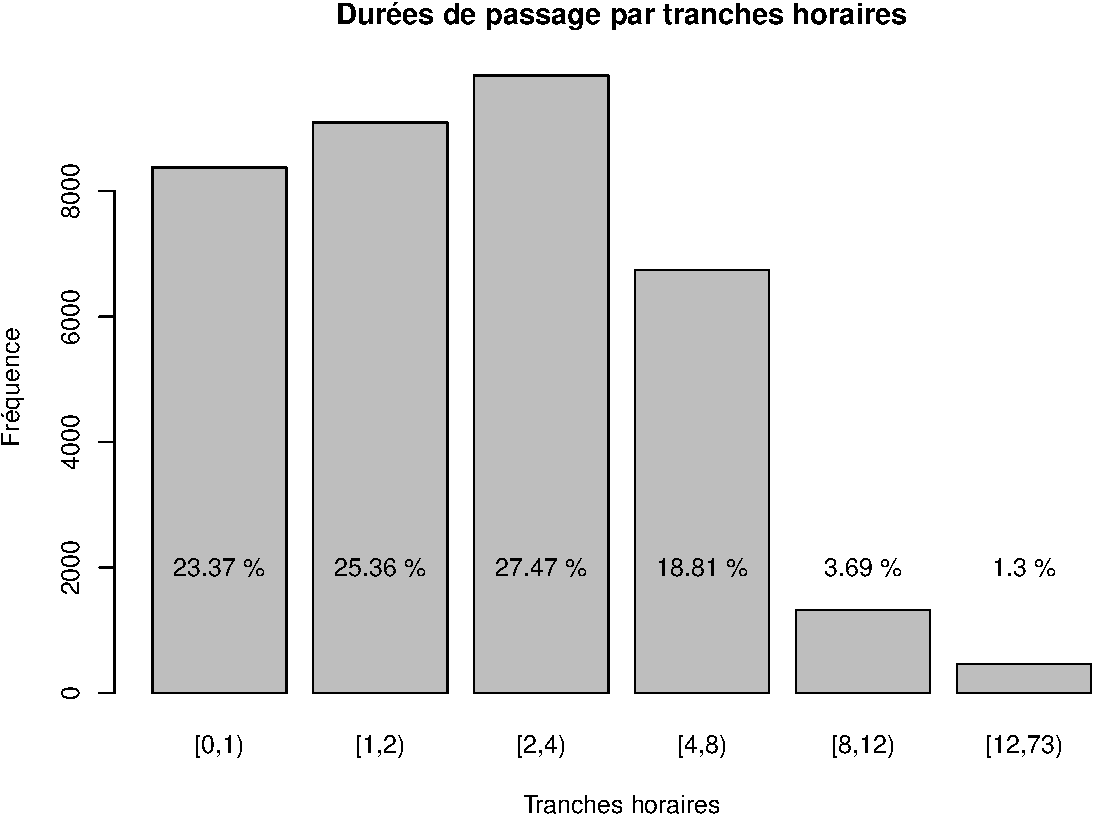
\includegraphics{rapport_2014_files/figure-latex/duree_tranches_horaires-1.pdf}
\end{itemize}

\section{Temps de calcul}\label{temps-de-calcul}

\begin{verbatim}
##    user  system elapsed 
##  30.446   1.076  32.026
\end{verbatim}

\begin{verbatim}
##                                                                            
## "2,014000e+03" "1,643600e+04" "1,646600e+04" "3,100000e+01" "1,000000e+00" 
##                                                                            
## "2,000000e+00" "1,300000e+01" "          NA" "          NA" "4,050900e+04" 
##                                                                            
## "1,306742e+03" "3,393600e+04" "6,573000e+03" "8,377398e-01" "1,622602e-01" 
##              F              M              F              M              M 
## "4,939360e+01" "5,060640e+01" "1,999700e+04" "2,048800e+04" "5,060640e-01" 
##                                                                            
## "1,991000e+03" "9,700000e+02" "4,915079e-02" "1,276900e+04" "3,152217e-01" 
##                                                                            
## "5,671000e+03" "1,399970e-01" "3,712992e+01" "2,780361e+01" "3,300000e+01" 
##              M              F 
## "3,533831e+01" "3,899030e+01"
\end{verbatim}

\end{document}
